\chapter{Discussion}
\section{Reliability of Test Results}
Providing a fully isolated test environment can be rather tricky. Due to this, there are a variety of factors that could affect the reliability of the test results. While trying out the same test cases at different times I noticed a framerate variance of around 3-8 FPS. There are a few possible explanations for why this happens. The first of these is the operating system's impact on general performance. Since the operating system can have different degrees of load on the hardware at different times, the related hardware interrupts that this brings can result in lower performance. In general, I tried to keep any additional programs closed during testing, but the operating system could still be doing tasks in the background, resulting in a performance loss. 

Another factor that could affect the performance is the overhead of the Unity Editor. This overhead should generally be consistent as the program was run without touching anything in the editor during testing. Regardless, there might still be some variable processing in the background that I am unaware of. 

The usage of a third party framerate counter provides a small amount of additional overhead to the tests. I do not believe that this is related to the framerate variance though as the overhead is consistent between all tests. The overhead itself should also be around 1 FPS from what I have observed with turning the framerate counter on and off. 
\section{Discussion Per Test Condition}
This section goes through the general thought process for the applied optimisations and includes some discussion on the various peculiarities that were found during testing. 

\subsection{Naive Unity}
This test condition was primarily meant to be a ''minimum effort'' example in terms of performance so it did not see that much testing. I made one test with TAA vs. SMAA for anti-aliasing as this was something that had an effect in the Job Optimised Unity condition. Given that this baseline already had very low framerate, using SMAA did at least allow for a FPS above 30 which could be considered acceptable by some. A game usually consists of more than a 37 FPS galaxy simulation though so its applicability at this level of performance is limited. 

\subsection{Job Optimised Unity}
\begin{figure}[tbph]
    \centering
    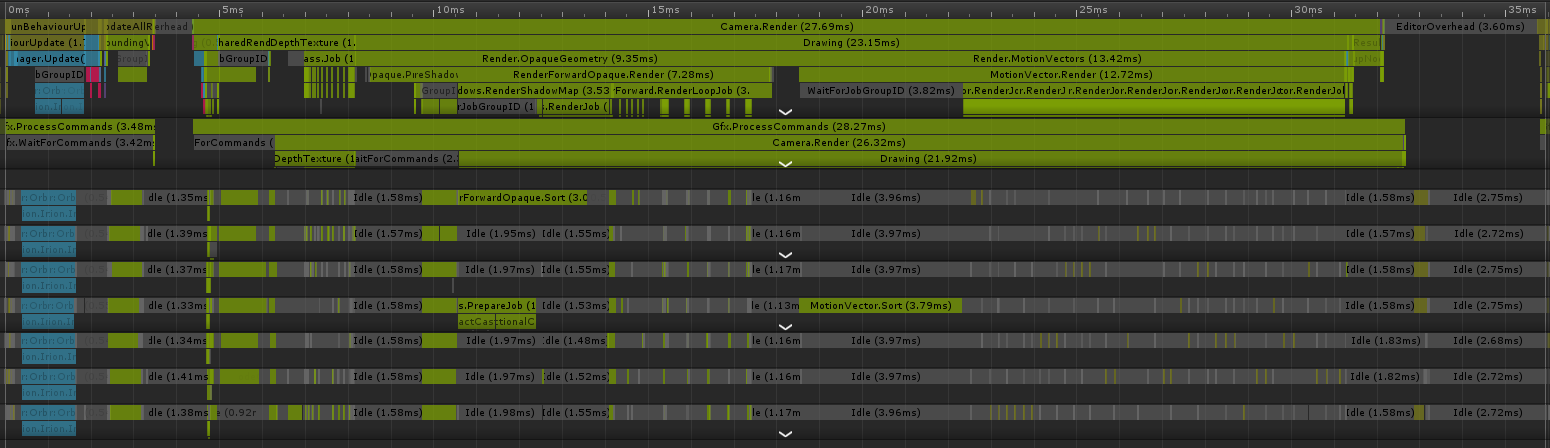
\includegraphics[width=1\textwidth]{Figures/JobUnityStandardFrame.png}
    \caption[Profiler frame from a Job Optimised Unity test]{Profiler frame from the TAA test in the Job Optimised Unity condition}
    \label{fig:joboptimisedtaaframe}
\end{figure}

After the initial implementation for this condition, I noticed that the biggest bottleneck in this case was graphics. This can be seen in Figure~\ref{fig:joboptimisedtaaframe} where the main thread mostly is occupied with graphics related tasks. To give some additional context on the image, the upper block consists of main thread usage while the lower block with large amounts of idle time is the usage of worker threads. One thing that stood out to me with this profiler frame was that MotionVectors took 13.42ms of the total frame time. MotionVectors in this case are used for the calculation of TAA which is why I made a new test where TAA is replaced by SMAA as this is a relatively simpler and cheaper anti-aliasing algorithm. This resulted in an increase from 32.7 FPS to 57.26 which is just shy of the 60 FPS that many view as the sweet spot for games. This does of course come at a trade-off in anti-aliasing quality, but given the overall small size of each star on screen, the difference should not be very noticeable. 

While working on the optimisations for this condition I was also experimenting with various ways to increase the performance of the Naive ECS condition. For ECS, making use of simpler meshes provided fairly large performance increases so I tried the same optimisation in this condition. Here, the performance results showed a small loss in FPS. I consider this as similar performance between sphere and cube meshes as the performance loss was within the variance range due to external factors.  

From this point and onwards, I was mostly working on both this and the Naive ECS condition to try and find new ways to improve performance. Graphics were generally still something that took a decent chunk of frame time so I tried various options from one of Unity's tutorials on graphics optimisation~\cite{unityPerformanceTutorial}. One of the changes I did was to switch to deferred rendering which resulted in a decent performance improvement (from 57 to 72 FPS). This comes with a few drawbacks which are mentioned in Section~\ref{sec:overalldisc}. 72 FPS is generally satisfactory in terms of framerate as it goes above 60, but the size of the galaxy itself still ended up being fairly small. 

\subsection{Naive ECS}
\begin{figure}[tbph]
    \centering
    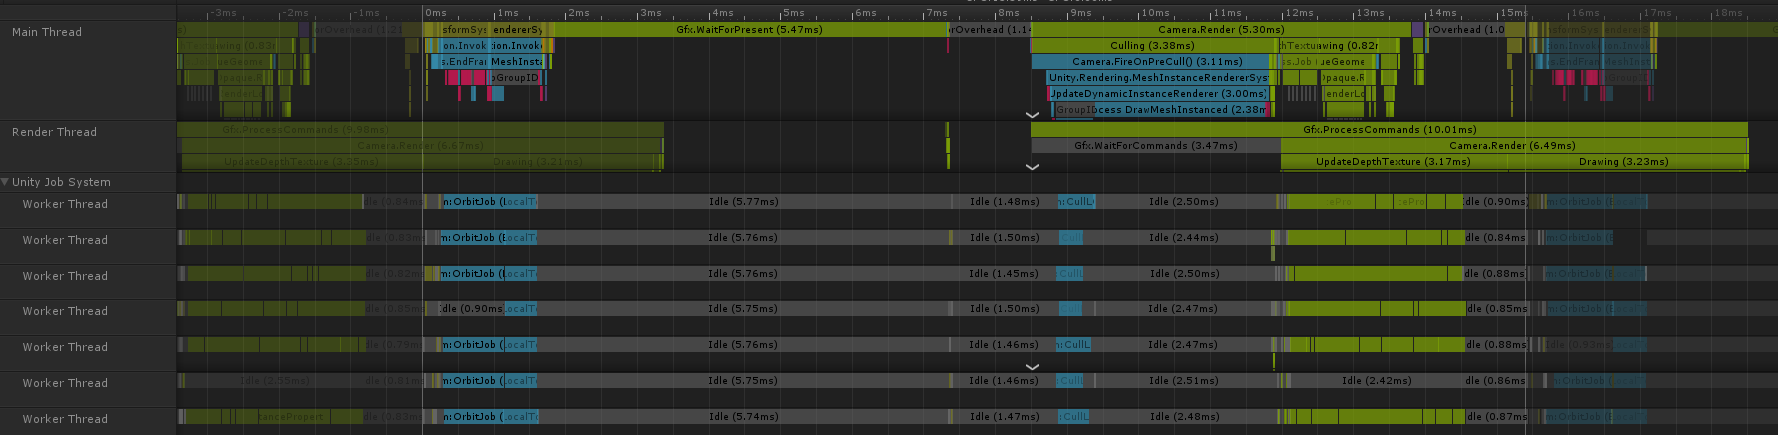
\includegraphics[width=1\textwidth]{Figures/NaiveECSStandardFrame.png}
    \caption[Profiler frame from a Naive ECS test]{Profiler frame from the TAA test in the Naive ECS condition}
    \label{fig:ecstaaframe}
\end{figure}

For the Naive ECS condition, graphics still took a sizeable chunk of the frame time, albeit not as much as the other conditions. This can be seen in Figure~\ref{fig:ecstaaframe}. Another apparent issue was the 5.47ms spent on Gfx.WaitForPresent which generally means that the CPU is waiting for the GPU to finish before moving on. I tried to make use of different forms of anti-aliasing like with the other conditions, but this did not seem to have any major effect with ECS. Due to this, I decided to stick with TAA for the Naive ECS condition as it is the more complex anti-aliasing method. An interesting performance increase came from using cube meshes for stars instead of spheres. Since this did not increase performance in the Job Optimised Unity condition it is a bit curious as to why it does so here. I suspected that this was a result of size differences in galaxies since the ECS galaxies consist of 60 000 stars by default instead of 10 000. Given the larger amount of stars, making use of simpler meshes reduces overall vertex counts which might affect performance to a larger degree.  

The largest performance increase for this condition came from using deferred rendering. The interesting thing about this is that once deferred rendering is used, mesh complexity no longer has any noticeable effect on performance (at least in terms of cube vs. sphere). It is rather hard to say why this is the case, but it could be that the simpler meshes worked well with forward rendering if the emissive material of the stars was used for lighting calculations. Given that the scene had a directional light, it could also be possible that lighting all the stars is more expensive for forward rendering at higher vertex counts. Deferred rendering is generally used to optimise performance with large amounts of lights, but it could also have helped in a scenario with only one. 

\section{Overall Discussion of Results}\label{sec:overalldisc}
In general, it is interesting to see how Unity ECS allows for ten times as many stars at similar framerates to the best Job Optimised Unity case. This is a fairly substantial difference in terms of GameObject/Entity sizes so why are the differences as big as they are? Part of the reason should be on the architectural side. Data-oriented design should generally allow for fairly good scalability compared to the object-oriented architecture with GameObjects. When there are a lot of GameObjects there should be a fair amount of cache misses as there are many callbacks and hierarchies to deal with per GameObject. On the rendering side, while both architectures interface with the same graphics API, there are differences in how the data is structured which also could further improve performance. 

Another thing to note is that all the ECS tests were compiled with the Burst compiler. I was originally under the impression that Burst only works with ECS Jobs, but it seems like it generally supports any job from the Job System. Due to this, it might be possible to further increase the performance of the Job Optimised Unity condition by adding Burst compilation, but I would not expect particularly major differences as many of the compiler optimisations are aimed at the ECS architecture. 

\subsection{Trade-offs for Deferred Rendering}
While deferred rendering has provided solid performance increases, its usage does come with some caveats. The first of these is the loss of MSAA which only works with forward rendering. MSAA is not a post-processing anti-aliasing algorithm like TAA or SMAA and requires the pipeline to be set up in a different way from how deferred rendering is structured. For this simulation, MSAA benefits Unity's bloom implementation to some degree as it reduces the overall flickering from moving objects with emissive materials. This flickering is less apparent with 100 000 stars as the bloom blends together due to the close proximities of stars, but it might become distracting with lower amounts of stars present. I have uploaded a short video to YouTube showcasing the difference at 60 000 stars here~\cite{msaabloom}. I would imagine that this trade-off could be worth the increase in performance, but that it depends on a case by case basis. At 100 000 stars, the flickering is not particularly noticeable so it works well there and the difference in general might not be as obvious unless you flick between using MSAA or not like in the video. Another option could be to use a different bloom implementation which has better anti-flicker functionality. 

Deferred rendering also comes with the trade-off of not being able to use regular alpha transparency for meshes, but this does not matter for the galaxy simulation as none of the stars are transparent. 

\subsection{Major Latency Spikes Throughout All Tests}
Throughout the tests a reoccurring theme is infrequent, but very large latency spikes. This is actually an issue with ECS that happens as long as the package is active/installed in a project. The culprit in this case is Unity's EndFrameTransformSystem which runs at the end of each frame. This is a known problem to Unity and Mike Acton who is one of the lead developers for ECS has mentioned that this will be fixed in the future~\cite{actonForum}. 

\section{Non-measured Test Cases}\label{sec:unrecordedcases}
Throughout the project, I briefly looked at some additional variables, but these were not measured due to time constraints. One of these is editor vs. release builds which was mentioned in Chapter~\ref{chap:methods}. It is rather strange how the performance drops so drastically even if the actual resolution is similar between the editor and the built release. I could not directly measure this problem either since my performance measurement script only works with the folder structure of the editor mode. Outside of ECS not necessarily being production ready yet, there might also be some specific quality settings that only apply in the release build. These settings could potentially impact performance.

Another non-measured test case is related to resolution. The test results were recorded at a lower resolution compared to the videos showing off some of the test cases. If we look at the 100 000 stars video~\cite{naiveECSVideo100k} then it shows an average of around 68 FPS while the test data resulted in \textasciitilde73 FPS. The resolution of the tests consisted of a 1047x589 viewport while the video has a 1616x909 viewport. If framerate variance and video recording overhead are taken into account, then the difference does not seem too large although this could change at higher resolutions. 
   
\section{Code Complexity vs. Performance Payoff}
One question that a developer might have when it comes to new functionality like ECS and the Job System is how much extra code complexity these result in. While it is not ideal, I have compiled the total lines of code and the total cyclomatic complexity for all three conditions using Visual Studio's code metrics in Figure~\ref{fig:cycloLines}.

\begin{figure}[tbph]
    \centering
    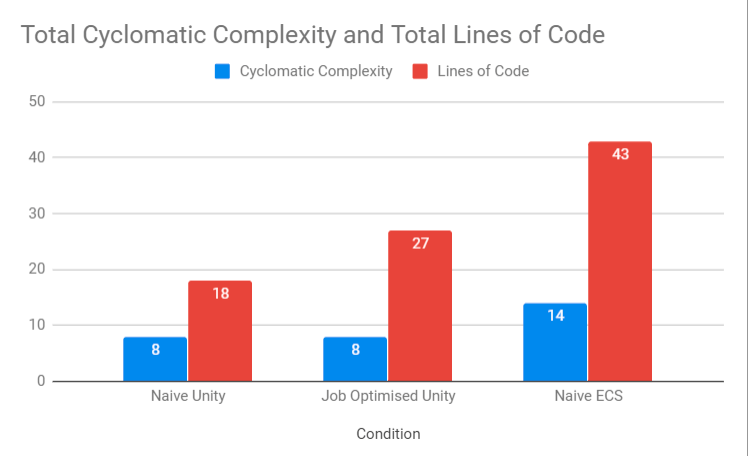
\includegraphics[width=0.75\textwidth]{Figures/cycloLines.png}
    \caption[Cyclomatic Complexity and Total Lines of Code per Condition]{Cyclomatic Complexity and Total Lines of Code per Condition}
    \label{fig:cycloLines}
\end{figure}

This can give a rough first impression for expected effort in terms of cyclomatic complexity and lines of code with this project as an example. This does of course not take into account the fact that a developer needs to learn and get used to the new technology which by itself could be considered a large leap in complexity. 

In terms of performance, moving from the best case Naive Unity to the best case Job Optimised Unity implementation results in a FPS increase of \textasciitilde92.519\%. Given that this only requires learning the Job System I think that this absolutely is worth doing as an optimisation. Learning how to use parallel jobs is generally something that will benefit a lot of developers in Unity and the added complexity from a static code analysis perspective is low. 

It is harder to compare performance with the Naive ECS condition as galaxy sizes vary, but it is worth mentioning that the best optimised ECS case can consist of ten times as many stars as the best Job Optimised Unity case (from 10 000 to 100 000). When working with ECS, a developer should expect to write more boilerplate code to get the highest performance gains and learning to work with data-oriented design might take some time. It is possible to work with hybrid solutions so that only the biggest bottlenecks are handled in ECS which could be useful. A hybrid solution will of course not yield the best performance though.

\section{The Future of Unity ECS}
While Unity ECS is currently in preview, it will soon see its first release during 2019. The expected lifetime of Unity ECS depends on user feedback, but it seems like Unity Technologies wants the ECS architecture to coexist with the existing object-oriented version. Since hybrid solutions also are possible at the moment, the fact that ECS does not contain as many official components and systems should not be an issue with initial releases. In terms of potential future replacements, I do not necessarily see anything that would replace the data-oriented workflow unless the way CPU's are architectured changes drastically in a manner that makes it less efficient.